\documentclass[12pt]{article}
\usepackage{anyfontsize}
\usepackage[margin = 2cm]{geometry}
\usepackage{polski}
\usepackage[utf8]{inputenc}
\usepackage{tabto}
\usepackage{graphicx}
\usepackage{amsmath}
\usepackage{multicol}


% Dot post number of section
\usepackage{titlesec}
% Underline section, dot post number and span post dot
\titleformat{\section}
    {\Large \bfseries}
    {\thesection.}
    {0.5 cm}
    {}[\titlerule\vspace{0.2cm}]
\titlelabel{\thetitle.\quad}


\usepackage{hyperref}
\hypersetup{
    colorlinks=true,
    linkcolor=black,
    filecolor=magenta,      
    urlcolor=cyan,
    pdfpagemode=FullScreen,
}

\usepackage{listings}


% \usepackage{csvsimple}
% \usepackage{pgfplots}

\usepackage[european, american currents, americanvoltages, RPvoltages, cute inductor]{circuitikz}
\usepackage{tikz}
\usetikzlibrary{shapes.geometric}

\title{\underline{Systemy mikroprocesorowe}\\\textbf{Dokumentacja projektu}\\Azor - The czołg}
\author{Piotr Kowol, Łukasz Przystupa}
\date{\today}


\usepackage{titling}
\renewcommand\maketitlehooka{\null\mbox{}\vfill}
\renewcommand\maketitlehookd{\vfill\null}

% \pgfplotsset{compat=1.18}

% \usetikzlibrary{shapes.geometric}


\begin{document}
    \maketitle
    \begin{center}
        Opiekun: Jacek Ostrowski
    \end{center}
    \thispagestyle{empty}
    \newpage


    \section*{Streszczenie}
    \tab Kilka słów podsumowujących pracę. Do napisania na \textbf{koniec}
    \thispagestyle{empty}
    \newpage
    
    \tableofcontents
    \newpage
    \section*{Wstęp}
\phantomsection
\addcontentsline{toc}{section}{\protect\numberline{}Wstęp}
    \tab Też do napisania potem

    \section{Cel i założenia projektowe}
    \tab Powyższy projekt oparty jest o mikrokontroler z rodziny AVR: ATmega8A.
    Komunikując się z odpowiedniki sensorami jest w stanie zlokalizować się w przestrzeni,
    oraz stworzyć prostą mapę pomieszczenia, w którym się znajduje. A następnie swobodnie poruszać się po nim.

    \subsection{Środowisko sprzętowe}
        \tab Jak wyżej wspomniano, sercem projektu jest mikrokontroler ATmega8A, a wspomnianymi modułami są odpowiednio:
        \begin{enumerate}
            \item Ultradźwiękowa czujka odległości -- HC-SR04,
            \item Trój-osiowy akcelerometr -- MMA8451,
            \item Moduł bluetooth -- HC05,
            \item Scalony mostek H -- układ L293D TexasInstruments,
            \item Silniki modelarskie z przekładniami 1:48 o napięciu znamionowym 6V,
            \item Serwo mechanizm -- SG-90,
            \item Trój-osiowy magnetometr QMC5883L.
        \end{enumerate}
% 
        Zasilanie dostarczają dwa wbudowane akumulatory litowo-jonowe 18650 o napięciu znamionowym 3.7V, podniesionym za pomocą przetwornicy STEP UP (CN6009) do około 5V.
        % Zasilanie jest z dwóch akumulatorów litowo-jonowych 18650 o napięciu znamionowym 3.7V, podniesionym za pomocą przetwornicy STEP UP do około 5V.

    \begin{figure}[!ht]
        \centering
        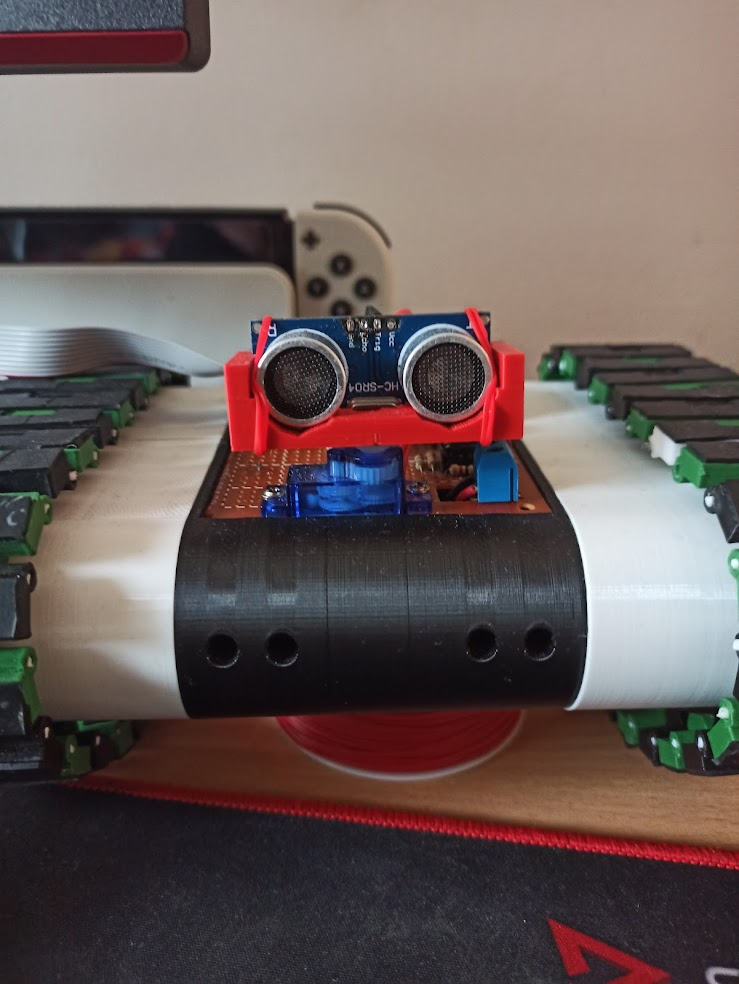
\includegraphics[height = 0.4\textheight]{Img/Azor.jpg}
        \caption{Zdjęcie „Azora”}
    \end{figure}

    \newpage
        \subsubsection{Schemat blokowy}
            \begin{figure}[!h]
    \centering
    \begin{circuitikz}
        \draw
            ( 0,  0) node [draw, rectangle, minimum width = 3cm, minimum height = 8cm](Atmega){ATmega}
            (-5,  1.75) node [draw, rectangle, minimum width = 3cm, minimum height = 2cm](HC_SR04){HC-SR04}
            (-5,  5) node [draw, rectangle, minimum width = 2cm, minimum height = 2cm](bt){HC05}
            ( 7,  1.5) node [draw, rectangle, minimum width = 2cm, minimum height = 2cm](com){QMC5883L}
            ( 7, -1.5) node [draw, rectangle, minimum width = 2cm, minimum height = 2cm](acc){MMA8451}
            ( 5,  4) node [draw, rectangle, minimum width = 2cm, minimum height = 1cm](eeprom){EEPROM}
            ( 5, -4) node [draw, rectangle, minimum width = 2cm, minimum height = 2cm](enkoder){Enkoder}
            
            (-5, -2) node [draw, rectangle, minimum width = 2cm, minimum height = 2cm](H_bridge){H Bridge}
            (-4, -5) node [draw, rectangle, minimum width = 2cm, minimum height = 2cm](servo){SG-90}
            (-7, -1.5) to[L] ++ (0, 1) -- ++ (1, 0) edge[bend left] ++ (0.5, -0.5)
            (-7, -1.5) -- ++ (1, 0)
            (-7, -3.5) to[L] ++ (0, 1) -- ++ (1, 0)
            (-7, -3.5) -- ++ (1, 0) edge[bend right] ++ (0.5, 0.5)

            % (3.25, -7) node [draw, rectangle, minimum width = 4cm, minimum height = 2cm, align=center, text width = 3cm](boostUp){Boost Up CN6009}
            % (-2.5, -7)node [draw, rectangle, minimum width = 2cm, minimum height = 2cm, text width = 2cm, align = center](BMS){Battery controller}
            % (0, -7.5) to[battery, invert] ++ (0, -1) node[ground]{}
            % (0, -7.5) -- ++ (-1.35, 0)
            % (0, -7.5) to[short, *-] ++ (1.3, 0)

            % (BMS) to[short, i=Enable] (boostUp)
            % (boostUp) ++(2, 0) -- ++(0.5, 0) -- ++ (0, 0.5) node[vcc]{$V_{CC}$}

            (eeprom) ++ (-0.5, -0.5) -- ++ (0, -5.5) -- ++ (1.4, 0)
            (eeprom) ++ ( 0,   -0.5) -- ++ (0, -5.0) -- ++ (0.9, 0)

            (com) ++ (-1.15, 0.5) to[short, -*] ++ (-0.85, 0) coordinate(sda)
            (com) ++ (-1.15, 0.0) to[short, -*] ++ (-1.35, 0) coordinate(scl)

            (sda) -- ++ (-1.5, 0) -- ++ (0, 1.5) coordinate(sda)
            (scl) -- ++ (-1.5, 0) -- ++ (0, 1.5) coordinate(scl)
            (sda) to[short] ++ (-2, 0)
            (scl) to[short] ++ (-1.5, 0)
            (sda) ++ (-1.25, 0) node[above]{SDA}
            (scl) ++ (-0.75, 0) node[below]{SCL}

            (sda) to[short, *-] ++ (0, 0.25) to[R] ++ (0, 2) node[vcc]{} ++ (-.25, 0.7) node[left]{$V_{CC}$}
            (scl) to[short, *-] ++ (0, 0.75) to[R] ++ (0, 2) node[vcc]{} ++ (0.25, 0.7) node[right]{$V_{CC}$}

            (bt) ++ (1, 0.25) to[short, i=RxD] ++ (2.00, 0) -- ++ (0, -1.75) -- ++ (0.50, 0)
            (bt) ++ (1,-0.25) to[short, i<_=TxD] ++ (1.75, 0) -- ++ (0, -1.75) -- ++ (0.75, 0)

            (HC_SR04) ++ (1.5, 0.25) to[short, i>=Echo] ++ (2.00, 0)
            (HC_SR04) ++ (1.5,-0.25) to[short, i<_=Trig] ++ (2.00, 0)

            (H_bridge) ++ (1, 0) to[short, i<=$\ $] ++ (1.5, 0) -- ++ (1, 0)

            (H_bridge) ++ (2.25, 0) node[above]{5}
            (H_bridge) ++ (2.25, 0) -- ++ ( 0.1,  0.1)
            (H_bridge) ++ (2.25, 0) -- ++ (-0.1, -0.1)

            (enkoder) ++ (-1, 0) -- ++ (-1, 0) -- ++ (0, 2) to[short, i>=$\ $] ++ (-1.5, 0)
            (servo) ++ (0.5, 1) -- ++ (0, 1) to[short, i<=$\ $] ++ (2, 0)
        ;
    \end{circuitikz}
    \caption{Schemat blokowy}
\end{figure}
    % \newpage
        
    \subsection{Środowisko programowe}
        \tab Program na ATmegę został napisany w języku C/C++, z wykorzystaniem bibliotek udostępnionych przez producenta.
        Do programowania, układu zostało wykorzystane narzędzie \textit{AVRdude} wraz z programatorem \textit{USBasp}.
        Natomiast graficzny interfejs dla komputerów klasy PC, został stworzony w Pythonie, z wykorzystaniem biblioteki ,,Turtle".

    \section{Interfejs komunikacyjny}
    \tab Wiele nowoczesnych urządzeń wykorzystuje rozmaite standardy i interfejsy komunikacyjne do różnych celów.
    Tak samo powyższy projekt wykorzystuje kilka prostych standardów do komunikacji zarówno z użytkownikiem oraz peryferiami.

    \subsection{Standard UART i interfejs bluetooth}
        \tab Podstawowym sposobem komunikacji z użytkownikiem jest protokół UART, wraz z interfejsem Bluetooth.
        Standard komunikacji UART, jest to prosty dwukierunkowy asynchroniczny sposób do przesyłania danych między dwoma urządzeniami.\\
        Opis przykładowej ramki w standardzie UART:
            
        \begin{figure}[!ht]
            \centering
            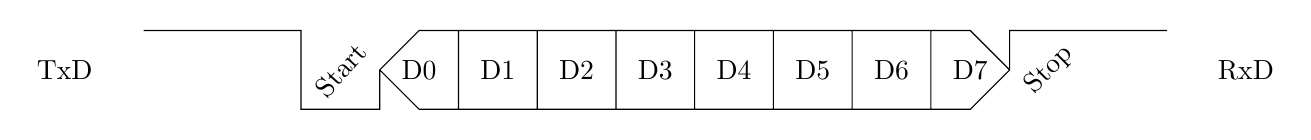
\begin{tikzpicture}
                \draw
                (-1, 0.5) node[]{TxD}
                (0, 1) -- (2, 1)
                    -- (2, 0)
                    -- (3, 0)
                    -- (3, 0.5) coordinate(start) ++(-0.5, 0) node[rotate = 48]{Start}

                (start) --++ (0.5, -0.5) -- ++ (7, 0) --++(0.5, 0.5) coordinate(stop)
                (start) --++ (0.5, 0.5) -- ++ (7, 0) --++(0.5, -0.5)

                (start) ++ (1, 0.5) -- ++ (0, -1) ++ (-0.5, 0.5) node[]{D0}
                (start) ++ (2, 0.5) -- ++ (0, -1) ++ (-0.5, 0.5) node[]{D1}
                (start) ++ (3, 0.5) -- ++ (0, -1) ++ (-0.5, 0.5) node[]{D2}
                (start) ++ (4, 0.5) -- ++ (0, -1) ++ (-0.5, 0.5) node[]{D3}
                (start) ++ (5, 0.5) -- ++ (0, -1) ++ (-0.5, 0.5) node[]{D4}
                (start) ++ (6, 0.5) -- ++ (0, -1) ++ (-0.5, 0.5) node[]{D5}
                (start) ++ (7, 0.5) -- ++ (0, -1) ++ (-0.5, 0.5) node[]{D6}
                (start) ++ (8, 0.5) ++ (0, -1) ++ (-0.5, 0.5) node[]{D7}
                % (start) ++ (8.5, 0) node[]{P}

                (stop) --++(0, 0.5) -- ++(2, 0) coordinate(end)
                (stop) ++ (0.5, 0) node[rotate = 45]{Stop}
                (end) ++ (1, -0.5) node[]{RxD}
                        
                ;
            \end{tikzpicture}
            \caption{Ramka danych w standardzie UART}
        \end{figure}
% 
        \noindent
        W tym projekcie komunikacja odbywa się z szybkością 9600baud'ów (Do zmiany prawie na 100\%).
        Dodatkowo, standard pozwala na przesyłanie dodatkowego bity parzystości ,,doklejanego" do końca wiadomości, jako sposób sprawdzania poprawności wysłanej wiadomości.

        Dalszą częścią kanału transmisyjnego jest przekaźnik bluetooth, który łączy się z komputerem na odpowiednim porcie szeregowym łatwym do oczytania dla programu napisanego na komputerze.
    
    \subsection{Interfejs Two Wire (I²C)}
        \tab Ostatnim interfejsem, wykorzystywanym przez „Azora” jest interfejs I$^2$C -- czyli dwukierunkowa szeregowa magistrala OC z układ Master-Slave.
        Standard ten służy do połączenie urządzeń peryferyjnych z kontrolerem.
        Komunikacja odbywa się w 8bitowych ramkach, z tym że pierwsza ramka zawsze definiuje adres urządzenia docelowego oraz określa kierunek transmisji „do”~lub~„z”~urządzenia.

        \begin{figure}[!ht]
            \centering
            \begin{circuitikz}
                \draw
                    (0, 0) node[draw, rectangle, minimum width = 2cm, minimum height = 2cm](Master){Master}
                    (0, -3.5) node[draw, rectangle, minimum width = 2cm, minimum height = 2cm](Slave1){Slave 1}
                    (2.5, -3.5) node[draw, rectangle, minimum width = 2cm, minimum height = 2cm](Slave2){Slave 2}
                    (5, -3.5) node[draw, rectangle, minimum width = 2cm, minimum height = 2cm](Slave3){Slave 2}

                    (0.25, -1.5) coordinate(clk) -- (5.5, -1.5) ++ (-1, 0) node[above]{$CLK$}
                    (0.25, -1.5) to[short, *-] ++ (0, 0.5) 
                        
                    (-0.25, -2.25) coordinate(sda) -- (5, -2.25) ++ (-1, 0) node[above]{$SDA$}
                    (-0.25, -2.25) to[short, *-] ++ (0, 1.25) 

                    ( 0.25, -1.5) -- ++ (0, -1)
                    (-0.25, -2.25) -- ++ (0, -0.25)
                        
                    (2.75, -1.5) to[short, *-] ++ (0, -1)
                    (2.25, -2.25) to[short, *-] ++ (0, -0.25)

                    (5.5, -1.5) to[short, -] ++ (0, -1)
                    (5.0, -2.25) to[short, -] ++ (0, -0.25)

                    (clk) -- ++ (-2.5, 0) to[R] ++ (0, 2) node[vcc]{+5V}
                    (sda) -- ++ (-3.0, 0) -- ++ (0, 0.75) to[R] ++(0, 2) node[vcc]{+5V}
                ;
            \end{circuitikz}
            \caption{Schemat blokowy magistrali I$^2$C}
        \end{figure}

\newpage
    \subsection{Interfejs SPI}
        % źródło: http://extronic.pl/content/60-kurs-xmega-interfejs-spi
        \tab Procesor bez programu, jest bezużytecznym kawałkiem krzemu dlatego niezwykle istotnym jest zaprogramowanie układu.
        Podstawową metodą programowania układów z rodziny ATmega jest interfejs SPI. 

        \begin{figure}[!ht]
            \centering
            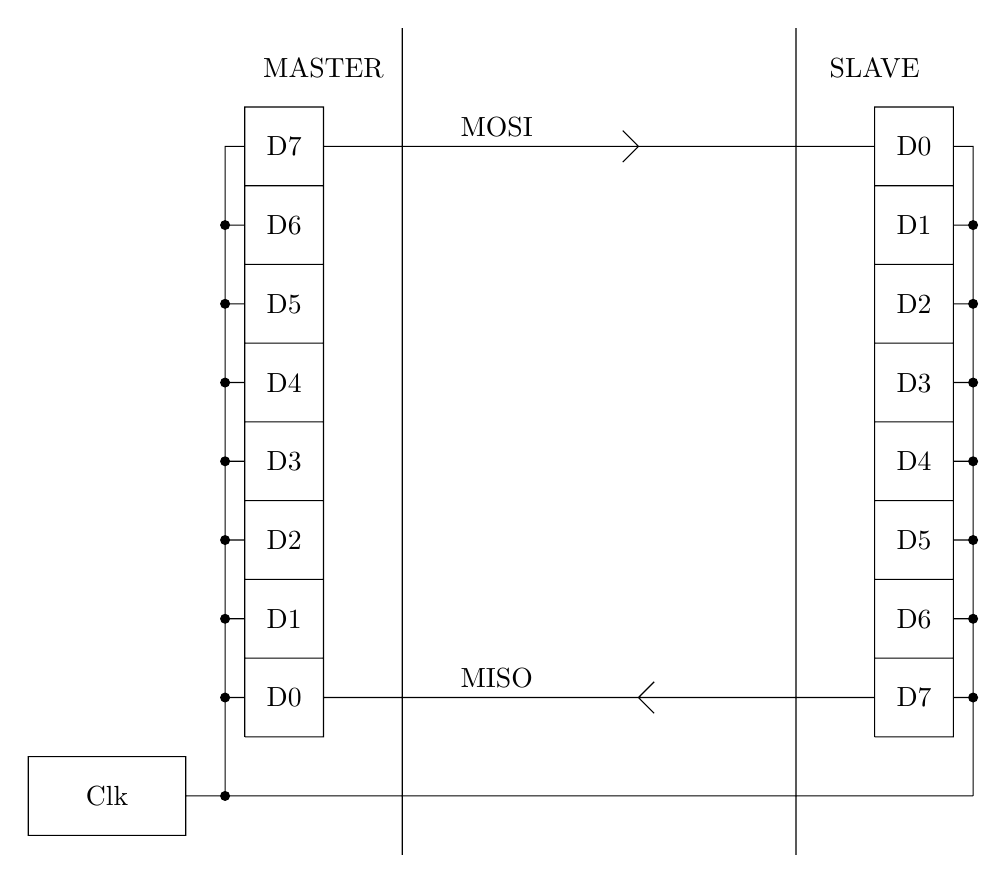
\begin{tikzpicture}
                \draw
                    (0, 0) -- (0, 8) -- (1, 8) -- (1, 0) -- (0, 0)
                    (0, 1) -- (1, 1) ++ (-0.5, -0.5) node[](MD0){D0}
                    (0, 2) -- (1, 2) ++ (-0.5, -0.5) node[]{D1}
                    (0, 3) -- (1, 3) ++ (-0.5, -0.5) node[]{D2}
                    (0, 4) -- (1, 4) ++ (-0.5, -0.5) node[]{D3}
                    (0, 5) -- (1, 5) ++ (-0.5, -0.5) node[]{D4}
                    (0, 6) -- (1, 6) ++ (-0.5, -0.5) node[]{D5}
                    (0, 7) -- (1, 7) ++ (-0.5, -0.5) node[]{D6}
                                        ++       (0, 1) node[](MD7){D7}
                    (2, -1.5) -- (2, 9)

                    (8, 0) -- (8, 8) -- (9, 8) -- (9, 0) -- (8, 0)
                    (8, 1) -- (9, 1) ++ (-0.5, -0.5) node[](SD7){D7}
                    (8, 2) -- (9, 2) ++ (-0.5, -0.5) node[]{D6}
                    (8, 3) -- (9, 3) ++ (-0.5, -0.5) node[]{D5}
                    (8, 4) -- (9, 4) ++ (-0.5, -0.5) node[]{D4}
                    (8, 5) -- (9, 5) ++ (-0.5, -0.5) node[]{D3}
                    (8, 6) -- (9, 6) ++ (-0.5, -0.5) node[]{D2}
                    (8, 7) -- (9, 7) ++ (-0.5, -0.5) node[]{D1}
                                        ++       (0, 1) node[](SD0){D0}
                    (7, -1.5) -- (7, 9)

                        
                    (-2.75, -1.25) rectangle ++ (2, 1)
                    (-1.75, -0.75) node[](clk){Clk} 
                    (clk) ++ (1, 0) coordinate(clk)
                    (clk) -- ++ (0.5, 0)
                        to[short, *-] ++ (0, 1.25) coordinate(MD)
                        to[short, *-] ++ (0.25, 0)
                    (MD) -- ++ (0, 1) coordinate(MD)
                        to[short, *-] ++ (0.25, 0)
                    (MD) -- ++ (0, 1) coordinate(MD)
                        to[short, *-] ++ (0.25, 0)
                    (MD) -- ++ (0, 1) coordinate(MD)
                        to[short, *-] ++ (0.25, 0)
                    (MD) -- ++ (0, 1) coordinate(MD)
                        to[short, *-] ++ (0.25, 0)
                    (MD) -- ++ (0, 1) coordinate(MD)
                        to[short, *-] ++ (0.25, 0)
                    (MD) -- ++ (0, 1) coordinate(MD)
                        to[short, *-] ++ (0.25, 0)
                    (MD) -- ++ (0, 1) coordinate(MD)
                        to[short] ++ (0.25, 0)

                    (clk) -- ++ (10, 0) coordinate(SD)
                    (SD) to[short, -] ++ (0, 1.25) coordinate(SD)
                        -- ++(-0.25, 0)
                    (SD) to[short, *-] ++ (0, 1) coordinate(SD)
                        -- ++(-0.25, 0)
                    (SD) to[short, *-] ++ (0, 1) coordinate(SD)
                        -- ++(-0.25, 0)
                    (SD) to[short, *-] ++ (0, 1) coordinate(SD)
                        -- ++(-0.25, 0)
                    (SD) to[short, *-] ++ (0, 1) coordinate(SD)
                        -- ++(-0.25, 0)
                    (SD) to[short, *-] ++ (0, 1) coordinate(SD)
                        -- ++(-0.25, 0)
                    (SD) to[short, *-] ++ (0, 1) coordinate(SD)
                        -- ++(-0.25, 0)
                    (SD) to[short, *-] ++ (0, 1) coordinate(SD)
                        -- ++(-0.25, 0)

                    (MD7) ++ (0.5, 0) coordinate (MD7)
                    (SD0) ++ (-0.5,0) coordinate (SD0)
                    (MD0) ++ (0.5, 0) coordinate (MD0)
                    (SD7) ++ (-0.5,0) coordinate (SD7)

                    (MD7) -- (SD0)
                    (MD0) -- (SD7)
                        
                    (MD7) ++ (4, 0) -- ++ (-0.2, 0.2)
                    (MD7) ++ (4, 0) -- ++ (-0.2, -0.2)
                    (MD7) ++ (2.2, 0) node[above]{MOSI}
                    % (SD7) ++ (-2.2, 0) node[above]{MISO}

                    (MD0) ++ (4, 0) -- ++ (0.2, 0.2)
                    (MD0) ++ (4, 0) -- ++ (0.2, -0.2)
                    (MD0) ++ (2.2, 0) node[above]{MISO}
                    % (SD0) ++ (-2.2, 0) node[above]{MOSI}

                    (MD7) ++ (0, 1) node[]{MASTER}
                    (SD0) ++ (0, 1) node[]{SLAVE}
                ;

            \end{tikzpicture}
            \caption{Schemat interfejsu SPI}
        \end{figure}
        \noindent
        W przeciwieństwie do poprzednio omawianego interfejsu,
        SPI jest interfejsem typu Master-Slave -- wyróżniamy układ sterujący (Master),
        którego zadaniem jest wyznaczenie taktowania zegara 
        oraz zarządzanie magistralą układami układami podrzędnymi (Slave), poprzez wystawienie stanu aktywnego na pinie \textit{,,CS"}.

        % Dodatkowo, urządzenia slave posiadają specjalne wejście ,,CS", których aktywacja zezwala na komunikację za pomocą protokołu SPI.
        

    \newpage
            

        
            
    \section{Metody pomiarowe}
    \subsection{Odległość -- dalmierz}
        \tab Podstawowym zadaniem „Azora” jest stworzenie mapy tereny.
        Proces ten wykonywany jest za pomocą dalmierza HC-SR04 zamocowane na serwo mechanizmie, dzięki czemu dalmierz może obracać się w osi Z od $0^\circ$ do $180^\circ$.\\
        Schemat połączenia:
        \begin{figure}[!h]
            \centering
            \begin{circuitikz}
                \draw
                    (0, 0) -- (0, -5)
                    (-2, 0) node[]{$\mu P$}

                    (3, -1.75) node[draw, rectangle, minimum width = 2cm, minimum height = 1cm](HC){HC-SR04}
                    (3, -4) node[draw, rectangle, minimum width = 2cm, minimum height = 1cm](SG){SG-90}

                    (0, -1.5) coordinate(ECHO) node[left]{(ECHO) PD4}
                    (0, -2.0) coordinate(TRIG) node[left]{(TRIG) PB6}
                    (0, -4.0) coordinate(PWM)  node[left]{(PWM) PB3}

                    (ECHO) -- ++ (2, 0)
                    (TRIG) -- ++ (2, 0)

                    (PWM) -- ++ (2, 0)

                    (HC) ++ (0, 0.5) node[vcc]{$V_{CC}$}
                    (SG) ++ (0, 0.5) node[vcc]{$V_{CC}$}

                    (HC) ++ (1, 0) node[ground]{}
                ;
            \end{circuitikz}
        \end{figure}

        \subsection{Algorytm działania:}
            \begin{figure}[!h]
                \centering
                \begin{circuitikz}
                    \draw
                        (0, 0) node [draw, circle, minimum width = 2cm, text width = 2cm, align=center]{Wysłanie sygnału TRIG}
                        (0, -4) node[draw, diamond, minimum width= 2cm, text width = 2cm, align=center]{Czy został odebrany sygnał z ECHO}
                    ;
                \end{circuitikz}
            \end{figure}

    \subsection{Prędkość -- enkoder}
    \subsection{Przyspieszenie -- akcelerometr}
    \subsection{Magnetometr -- cyfrowy kompas}
    \section{Interfejs użytkownika}
    Oprogramowanie pozwala na komunikację z „Azorem” oraz reprezentację danych pomiarowych. Po uruchomieniu 
    programu należy w CLI wybrać port szeregowy, wykorzystywany do komunikacji przez moduł Bluetooth, aby nawiązać
    łączność z „Azorem”.\\
    Okno interfejsu graficznego można podzielić na trzy obszary:
    \begin{itemize}
        \item mapa skanowanego obszaru
        \item radar ukazujący obecne pole widzenia „Azora”
        \item przyciski do sterowania „Azorem”
    \end{itemize}
    \subsection{Podstawowe sterowanie „Azorem”}
        Interfejs graficzny posiada panel sterowania z przyciskami funkcyjnymi pozwalającymi na przemieszczanie 
        i obracanie „Azora” oraz służące do obracania czujnika odległości i wykonywania pojedynczych pomiarów. 
        Przyciski przód/tył umożliwiają przemieszczenie robota o około 100 mm w odpowiednim kierunku. Strzałki 
        prawo/lewo pozwalają na jego obrót o $90^\circ$ w odpowiednią stronę, a zagięte strzałki w prawo/lewo 
        umożliwiają obracanie czujnikiem odległości z krokiem $15^\circ$. Położenie „Azora” na mapie jest 
        reprezentowane za pomocą niebieskiego kursora, a obrót „głową” jest pokazany na radarze za pomocą białego 
        kursora. Wykonanie pojedynczego pomiaru umożliwia okrągły przycisk znajdujący się na środku panelu sterowania. 
        Aby wykonać automatyczny cykl skanowania, należy kliknąć na radar. Spowoduje to automatyczne obracanie 
        czujnikiem odległości z krokiem $3^\circ$ i zapisywanie danych pomiarowych.
    \subsection{Reprezentacja danych}
        Dzięki możliwości obracania czujnikiem odległości w zakresie $0^\circ-180^\circ$, „Azor” może skanować
        półkole o promieniu 720 mm. Wyniki pojedynczego cyklu skanowania są wyświetlane na radarze, znajdującym się
        z lewej strony interfejsu użytkownika.\\
        Na podstawie zebranych danych i obecnego położenia „Azora” zostaje nakreślona mapa obszaru.
    \subsection{Zaawansowane sterowanie}
        Oprócz sterowania za pomocą przycisków istnieje możliwość wysyłania poleceń do „Azora” za pośrednictwem CLI. 
        W tym celu zostały stworzone odpowiednie komendy:
        \begin{itemize}
            \item \textit{forward [wartość]} - przemieszczenie „Azora” w przód o podaną odległość w mm, 
            domyślna wartość to 100 mm
            \item \textit{backward [wartość]} - przemieszczenie „Azora” w tył o podaną odległość w mm, 
            domyślna wartość to 100 mm
            \item \textit{left [wartość]} - obrót „Azora” w lewo o podany kąt, wartość domyślna to $90^\circ$
            \item \textit{right [wartość]} - obrót „Azora” w prawo o podany kąt, wartość domyślna to $90^\circ$
            \item \textit{head left/right [wartość]} - obrót czujnikiem odległości w lewo/prawo o podany kąt,
            wartość domyślna to $6^\circ$
            \item \textit{head set [wartość]} - obrót głową „Azora” do zadanego kąta z zakresu $0^\circ-180^\circ$,
            domyślnie $90^\circ$, co oznacza „patrzenie” w przód
            \item \textit{head measure} - wykonanie pomiaru odległości dla obecnego ustawienia czujnika odległości
            \item \textit{acc} - ???
            \item \textit{magnet} - ???
            \item \textit{azimuth} - ???
            \item \textit{distance} - ???
            \item \textit{time} - ???
            \item \textit{velocity} - ???
            \item \textit{radar} - wykonanie automatycznego pomiaru odległości w zakresie $0^\circ-180^\circ$ z krokiem $3^\circ$
            \item \textit{exit} - zakończenie działania programu
        \end{itemize}

\end{document}